\documentclass[a4paper,11pt]{article}

\usepackage[T1]{polski}
\usepackage[utf8]{inputenc} 
\usepackage{graphicx}
\usepackage{float}
\usepackage{verbatim}
\usepackage[obeyspaces]{url}
\usepackage{hyperref}
\usepackage{xcolor}
\usepackage{lastpage}
\usepackage{fancyhdr}
\usepackage{enumitem}
\usepackage{titling}
\usepackage{adjustbox}
\usepackage{array}
\usepackage{changepage}
\usepackage{booktabs}

\newcolumntype{R}[2]{%
	>{\adjustbox{angle=#1,lap=\width-(#2)}\bgroup}%
	l%
	<{\egroup}%
}
\newcommand*\rot{\multicolumn{1}{R{90}{1em}}}
\renewcommand\maketitlehooka{\null\mbox{}\vfill}
\renewcommand\maketitlehookd{\vfill\null}

\pagestyle{fancy} 
\fancyhf{}
\renewcommand{\headrulewidth}{0pt} 

\cfoot{\thepage \hspace{1pt} z \pageref*{LastPage}}
\rfoot{\hyperlink{toc}{Spis treści}}

\hypersetup{
    colorlinks,
    linkcolor={black},
    filecolor={blue}
}

\newcommand{\linkToFile}[2]{\href[pdfnewwindow=true]{#1}{\nolinkurl{#2}}}

\title{ Symulator inteligentnego sterowania windą \\ Sprawozdanie}
\author{Artur Gajowniczek \\ Michał Kośmider \\ Michał Kalisiak \\ Karol Mąkosa \\ Rafał Woźniak}

\begin{document}
\begin{titlingpage}
\maketitle
\end{titlingpage}
\thispagestyle{empty}
\cleardoublepage

\setcounter{page}{1}

\hypertarget{toc}{}
\tableofcontents

\cleardoublepage

\section{Wprowadzenie}
Systemy wbudowane i czasu rzeczywistego znajdują w dzisiejszym świecie coraz więcej zastosowań. Nowoczesna technologia przyzwyczaiła ludzi do bardzo krótkiego czasu odpowiedzi w niemalże wszystkich systemach komputerowych. Powstało też wiele systemów, w których z góry określony czas odpowiedzi jest kluczowy dla ich poprawnego działania i to właśnie one są nazywane systemami czasu rzeczywistego. Systemy wbudowane natomiast są nierozerwalnie połączone z urządzeniem, które obsługują. Jednym z przykładów systemu, który jest jednocześnie systemem wbudowanym oraz czasu rzeczywistego, jest system inteligentnego sterowania windą.
\\
\\
Problem, który rozwiązuje system sterowania windą jest w dużym stopniu podobny do dobrze znanego Problemu Komiwojażera, jednak występuje kilka znaczących różnic między nimi. Główną różnicą jest fakt, że w Problemie Komiwojażera całe zadanie jest od początku znane, natomiast w naturalnym środowisku windy warunki zadania cały czas się zmieniają, ponieważ pojawiają się nowi ludzie. Z tego powodu nie można z góry wyliczyć optymalnego rozwiązania, algorytm sterowania musi brać pod uwagę zmiany przy podejmowaniu kolejnych decyzji.

\section{Istniejące rozwiązania}
Inteligentne sterowanie windą nie jest nowym problemem i został już opracowany niejeden algorytm z nim związany. Większość z nich zajmuje się sterowaniem grupą wind, a nie pojedynczą windą. Poniżej znajduję się lista kilku z tych algorytmów oraz strategii wraz z krótkimi opisami.

\begin{itemize}
\item Strategia kontroli kolektywnej [1] -- w tym algorytmie winda porusza się w jednym kierunku zabierając tylko pasażerów jadących w tym samym kierunku. Gdy wszyscy pasażerowie wysiądą i nie ma następnych pasażerów znajdujących się dalej w danym kierunku niż winda, winda zmienia kierunek jeśli są jakieś inne wezwania. W przeciwnym wypadku winda będzie czekać na piętrze na którym wysiadł ostatni pasażer.
\item Strategie przeszukujące [1] -- w odróżnieniu od poprzedniej strategii, która należy do rodziny algorytmów zachłannych, strategie przeszukujące będą analizować wiele (lub wszystkie) możliwości i ich konsekwencje, a następnie podejmować decyzje wybierając spośród możliwości tę, która najlepiej spełnia zadane kryterium optymalizacyjne np. średni czas oczekiwania, średni czas obsłużenia, itp.. Strategie przeszukujące potrzebują więcej czasu na podjęcie decyzji, co może negatywnie wpływać na na średni czas oczekiwania, ale całościowo wyniki będą lepsze.
\item Strategia oparta na regułach [1] -- jest to strategia oparta na weryfikacji logicznych zdań typu ,,JEŚLI warunek TO skutek''. Takie reguły są tworzone na podstawie wiedzy ekspertów oraz przeprowadzanych badań.
\item Algorytm genetyczny [1] -- używając algorytmu genetycznego system sterujący windą, może ,,nauczyć się'' reagować na różne sytuacje poprzez ustawienie funkcji przystosowania zachowania jako funkcji optymalizowanego parametru np. średniego czasu oczekiwania.
\item Model zużycia energii [2] -- jest to model oparty o optymalizację przejechanych pięter do rozwiezienia wszystkich pasażerów w danej chwili czasowej.
\end{itemize}

\section{Opis architektury programu}
Symulator inteligentnego sterowania windą w naszym projekcie został zaimplementowany przy użyciu języka \textbf{Java} w wersji 8. Dodatkowo użyta została biblioteka do interfejsu graficznego użytkownika -- \textbf{JavaFx}.\\~\\
Działanie programu można podzielić na kilka niezależnych, lecz połączonych interfejsami modułów.
\subsection{Moduł interfejsu graficznego}
Użycie biblioteki \textbf{JavaFx} pozwoliło na uzyskanie ładnego okna graficznego, które prezentuje przejrzysty interfejs.\\~\\

\begin{figure}[H]
    \centering
    \caption{Okno główne}
    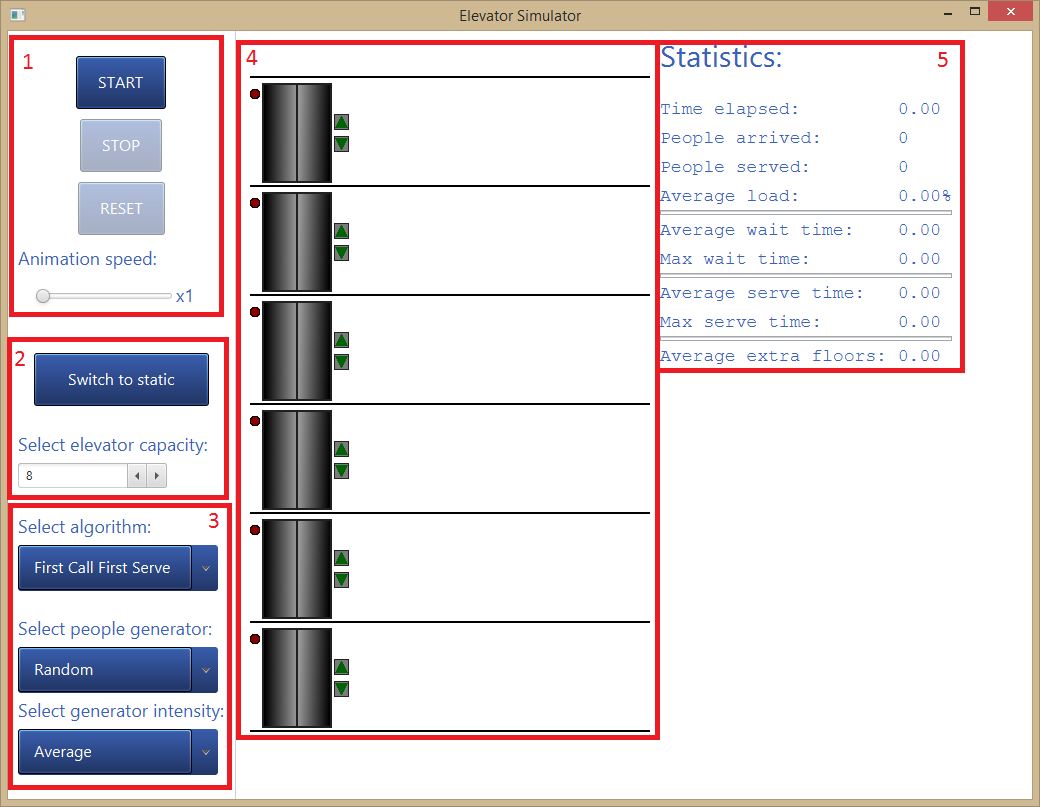
\includegraphics[width=\textwidth]{okno.png}
\end{figure}

\begin{enumerate}
	\item Przyciski sterujące rozpoczęciem i zakończeniem pracy windy, zresetowaniem windy do stanu początkowego oraz suwak służący do przyspieszania animacji
	\item Przyciski zmieniające tryb pracy generatora ludzi (statyczny i dynamiczny) oraz ustawiający maksymalną pojemność windy
	\item Rozsuwane listy wyboru algorytmu sterowania windą oraz wyboru generatora ludzi i jego intensywności generacji (tylko w przypadku trybu dynamicznego)
	\item Obszar prezentujący aktualny stan windy
	\item Obszar zawierający statystyki
\end{enumerate}
\subsection{Moduł kontroli windy}
Zajmuje się przechowywaniem oraz modyfikacją aktualnego stanu windy za pomocą maszyny stanów. Przechowuje on także informacje o ludziach znajdujących się na poszczególnych piętrach oraz w windzie.  Generuje zdarzenia, które dopisywane są do kolejki zdarzeń w module zegara.
\subsection{Moduł zegara}
Zarządza zdarzeniami z poszczególnych modułów, które dzięki działaniu zegara, odbywają się w predefiniowanych chwilach czasowych. Każde zdarzenie w systemie zajmuje określoną liczbę tyknięć zegara, co symuluje upływ czasu (na przykład przejechanie piętra trwa dłużej niż otworzenie drzwi).
\subsection{Moduł generacji ludzi}
Pozwala na generowanie ludzi chcących skorzystać z windy na różne sposoby. Każdy z algorytmów bazuje na rozkładzie Poissona, którego parametr lambda można modyfikować przy użyciu interfejsu graficznego (poprzez zmianę intensywności generatora). Zaimplementowane metody generowania ludzi to:
\begin{itemize}
	\item Random -- algorytm losowy, żadne piętro nie jest faworyzowane w tym algorytmie, ludzie pojawiają się na wszystkich piętrach z takim samym prawdopodobieństwem i chcą jechać na losowe, inne piętra
	\item Office Morning -- symuluje napływ ludzi do biurowca w godzinach porannych. Najwięcej ludzi pojawia się na parterze, natomiast na innych piętrach ludzie pojawiają się sporadycznie
	\item Office Evening -- symuluje wychodzenie ludzi z biurowca w godzinach popołudniowo-wieczornych. Ludzie na parterze pojawiają się sporadycznie, natomiast na pozostałych piętrach ludzie pojawiają się z takim samym prawdopodobieństwem i wszyscy chcą jechać na parter
\end{itemize}
\subsection{Moduł algorytmów sterowania windą}
Pozwala na wybór algorytmu służącego do podejmowania decyzji przez moduł kontroli windą. Zaimplementowane algorytmy to:
\begin{itemize}
	\item First Call First Serve -- obsługuje pierwsze zgłoszone żądanie, z wyjątkiem sytuacji, gdy po drodze jest w stanie obsłużyć jakieś inne żądanie
	\item Momentum -- realizuje strategię kontroli kolektywnej
	\item Morning -- stara się zoptymalizować czas oczekiwania w biurowcu w godzinach porannych, poprzez zjeżdżanie na parter w przypadku bezczynności windy
\end{itemize}
\subsection{Moduł statystyk}
Zajmuje się wyliczaniem statystyk widocznych w obszarze statystyk. Są to (każda statystyka określająca czas jest wyrażona w tyknięciach zegara):
\begin{itemize}
	\item Elapsed time -- czas, który upłynął od rozpoczęcia symulacji
	\item People arrived -- liczba ludzi, która pojawiła się w sumie na wszystkich piętrach od rozpoczęcia symulacji
	\item People served -- liczba ludzi, która została obsłużona od rozpoczęcia symulacji
	\item Average load -- średnie obciążenie windy wyrażone jako procent jej pojemości od rozpoczęcia symulacji
	\item Average wait time -- średni czas oczekiwania ludzi zanim mogli wsiąść do windy
	\item Max wait time -- najdłuższy czas oczekiwania osoby zanim mogła wsiąść do windy
	\item Average serve time -- średni czas obsłużenia ludzi (od pojawienia się na piętrze początkowym, do dotarcia na piętro docelowe)
	\item Max serve time -- najdłuższy czas obsłużenia osoby
	\item Average extra floors -- średnia liczba pięter przejechanych ponad najmniejszą możliwą liczbę pięter dla każdego pasażera
\end{itemize}

\section{Testowanie statyczne}
Zaczęliśmy od przetestowania algorytmów w wersji statycznej, to znaczy ludzie byli wygenerowani na samym początku symulacji, a w później generator był wyłączony i nowi ludzie nie pojawiali się. Winda zaczynała zawsze z parteru. Rozkład ludzi na którym testowaliśmy algorytmy to:
\begin{itemize}
\item 1 osoba na parterze chcąca jechać na piąte piętro
\item 2 osoby na pierwszym piętrze, z których jedna chce jechać na trzecie piętro, a druga na parter
\item 6 osób na trzecim pięrze, z których jedna chce jechać na pierwsze piętro, a pozostałe na piąte piętro
\end{itemize}


\section{Bibliografia}
[1] https://www.diva-portal.org/smash/get/diva2:668654/FULLTEXT01.pdf
[2] http://www.csc.kth.se/utbildning/kth/kurser/DD143X/dkand13/Group3Johan/report/\\
\indent alexandra.nordin.frederick.ceder.report.pdf

\end{document}